%!TEX root = ../report.tex
\chapter{Experiments}
\label{experiments}
In this chapter the experimental results are presented. The experimental method is outlined in chapter~\ref{method}. 

\section{Map 1: IranOpen 2012 - Pre 2}
This map was used in the Iran Open 2012 competition \cite{iran2012}. The map features a grey hospital-like environment with grey tiled floors and walls. In figure~\ref{fig:map1} a screenshot of the environment is shown along with the map after the Weighted Scan Matcher was run on the simulation data. 

\begin{figure}[ht]
\centering
\subfigure[Screenshot]{
	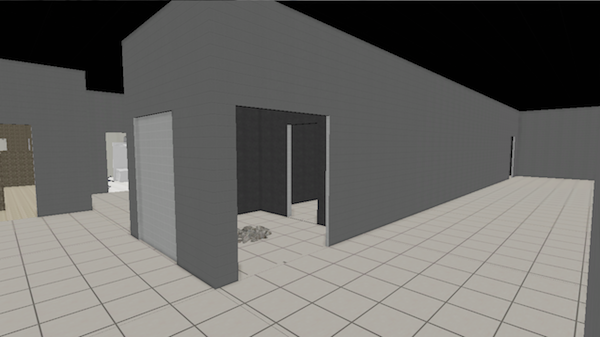
\includegraphics[width=0.5\textwidth]{images/experiment/map1/screenshot.png}
	\label{fig:map1-screenshot}
}
\subfigure[Map created with the Weighted Scan Matcher]{
	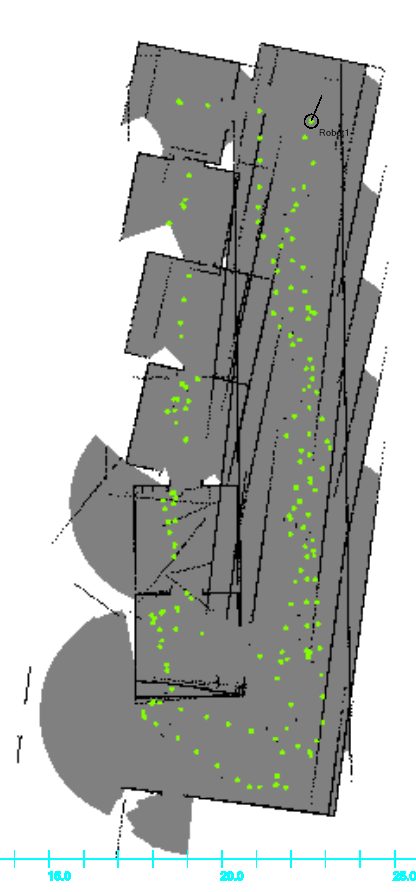
\includegraphics[width=0.3\textwidth]{images/experiment/map1/slam.png}
	\label{fig:map1-map}
}
  \caption{The ground truth, inertia sensor and slam path of the robot on a piece of map 1.}
  \label{fig:map1}
\end{figure}

The map shows a lot of noise and errors. As can be seen in figure~\ref{fig:apx:map1-paths} (in the appendix), the inertia sensor gives a rather good location-estimate, but the rotation estimate from position 160 onwards is off by more than $10\degree$. The scanmatcher fails regularly because it takes the inertia sensor location estimate as begin point for its search. When the location according to SLAM and inertia sensor diverge too far, the SLAM matcher fails -- it only searches a local neighborhood around the initial seed pose given by the inertia sensor. The result of this is a map with jagged lines, as can be seen in figure~\ref{fig:map1-map} and figure~\ref{fig:map1}.

\begin{figure}[ht]
  \centering
  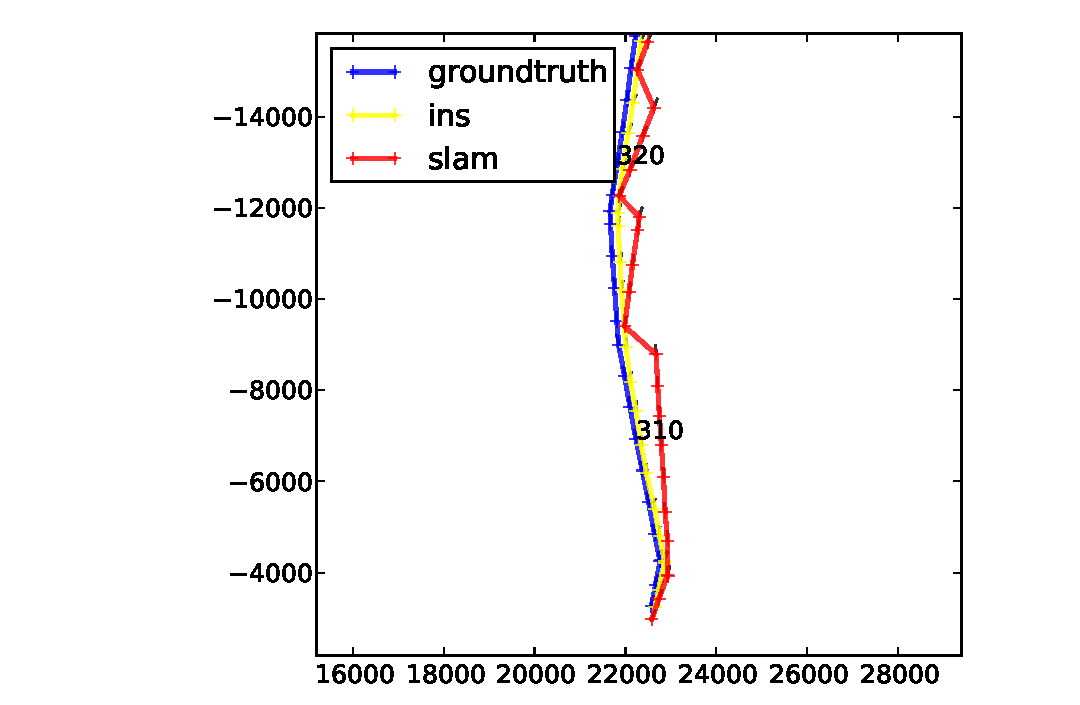
\includegraphics[width=0.7\textwidth]{images/experiment/map1/ins-problem.pdf}
  \caption{A small part of the path the robot moved in map 1. The wrong rotation estimate of the inertia sensor (yellow line) makes the slam-matcher (red line) think the robot moved in another direction than it did in reality (blue line). When the inertia sensor reading and SLAM result diverge too far, the SLAM location is reset to the inertia sensor estimate. This results in a jagged path estimate from the SLAM sensor.}
  \label{fig:map1-ins-problem}
\end{figure}


\subsection{Segmenting the map}
The confidence measures of the first map are shown in figure~\ref{fig:map1-confidence-measures-vs-time}. It is immediately apparent that the extreme values of the three metrics coincide. When the scan matcher matches few scanlines, the determinant and trace values are at their maximum. When the scan matcher matches no scanlines, the determinant and trace of the covariance matrix are undefined. These show up as red dots on the x-axis. When the scan matcher matches many scanlines, its increased confidence in a correct match is reflected in a covariance matrix with small determinant and trace.

In figure~\ref{fig:map1-confidence-measures-scatter} the values of the three confidence measures are plotted against each other to emphasize their correlation. The (Spearman) rank correlation gives an indication how well the relationship between the two variables can be described by a monotonic function. The spearman rank correlation coefficients between the confidence measures is as follows. Between trace and determinant $0.85$, between number of matches and determinant $-0.50$, and between number of matches and trace $-0.48$, all with a p-value $\ll 10^{-10}$. This means that all three confidence measures are strongly correlated.

\begin{figure}[ht]
  \centering
  \subfigure[Confidence measures through time]{
    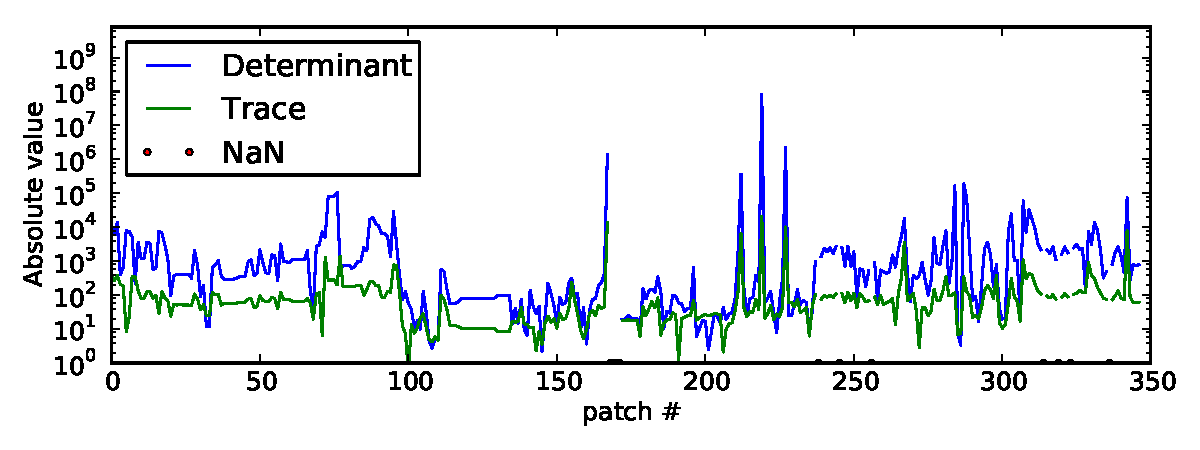
\includegraphics[width=\textwidth]{images/experiment/map1/error-measures.pdf}
    \label{fig:map1-confidence-measures-vs-time}
  }
  \subfigure[Scatter plot between the three confidence measures.]{
    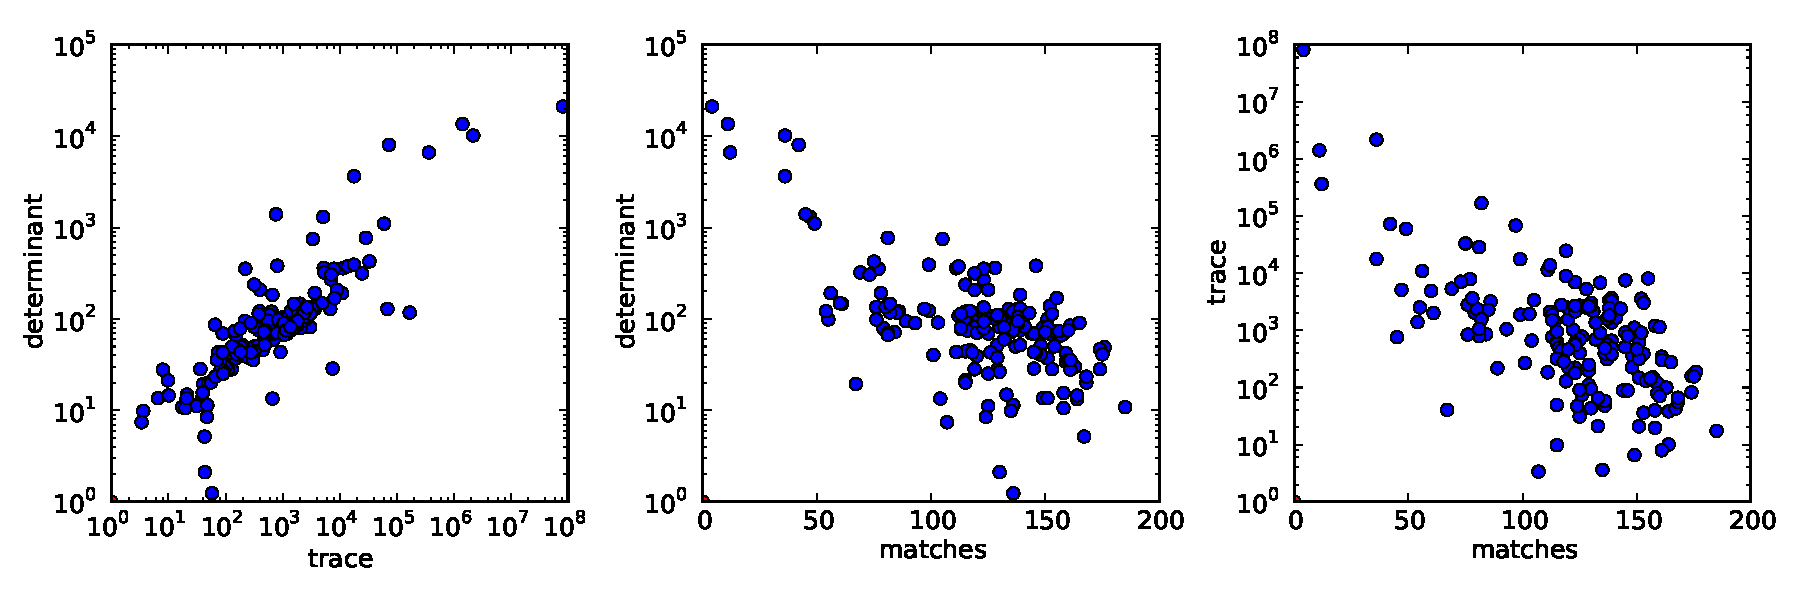
\includegraphics[width=\textwidth]{images/experiment/map1/error-measures-scatter.pdf}
    \label{fig:map1-confidence-measures-scatter}
  }
  \caption{Confidence measures for map 1.}
  \label{fig:map1-confidence-measures}
\end{figure}

When there are no matches at all, the scanmatcher has failed most spectacularly. In that case, the covariance matrix can not even be computed. In extention, the determinant or trace of the covariance matrix can not be computed either. This occurs at the following timesteps: 66  67  68  96 103 113 159 164 168 175. The greatest rift lies at $66 \le t \le68$, where there were 3 consecutive timesteps that could not be matched. The submaps that are procured can be found in the appendix, figure~\ref{fig:apx:map1-pieces}. 

\subsection{Stitching}
The Hough map stitching procedure as outlined in chapter~\ref{chapter:hough} between the first two sub-maps results in an optimal rotation $\theta_1$ of $13\degree$, with a much less pronounced secondary hypothesis $\theta_2$ of $103\degree$, as can be seen in figure~\ref{fig:exp:1:theta}. The X- and Y-spectra for $\theta_{1a}$ are shown in figure~\ref{fig:exp:1:xy}. The resulting map is shown in figure~\ref{fig:exp:1:result1}.

\begin{figure}[ht]
  \centering
  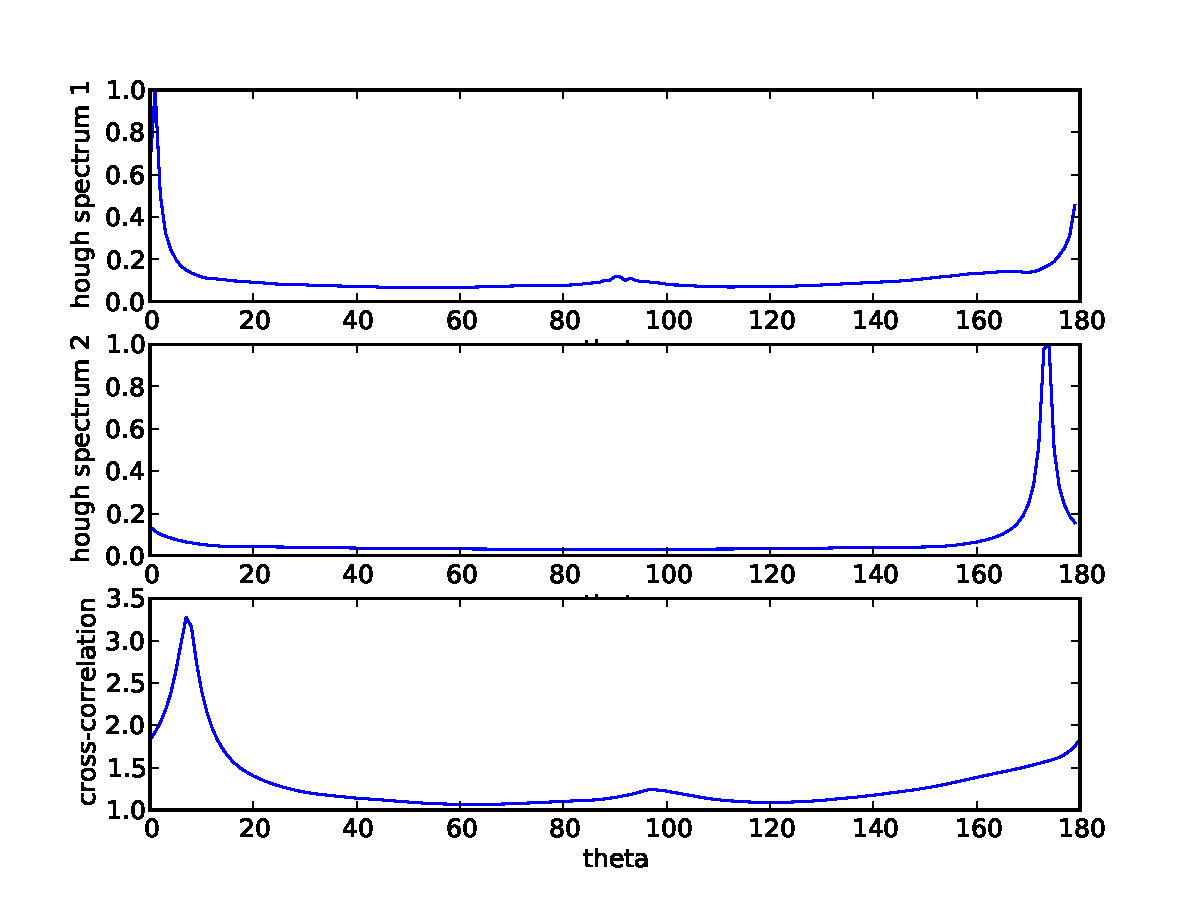
\includegraphics[width=0.8\textwidth]{images/experiment/map1/stitch1-theta-correlation-result.pdf}
  \caption{Finding optimal rotation $\theta$ through correlating Hough spectra.}
  \label{fig:exp:1:theta}
\end{figure}

\begin{figure}[ht]
  \centering
  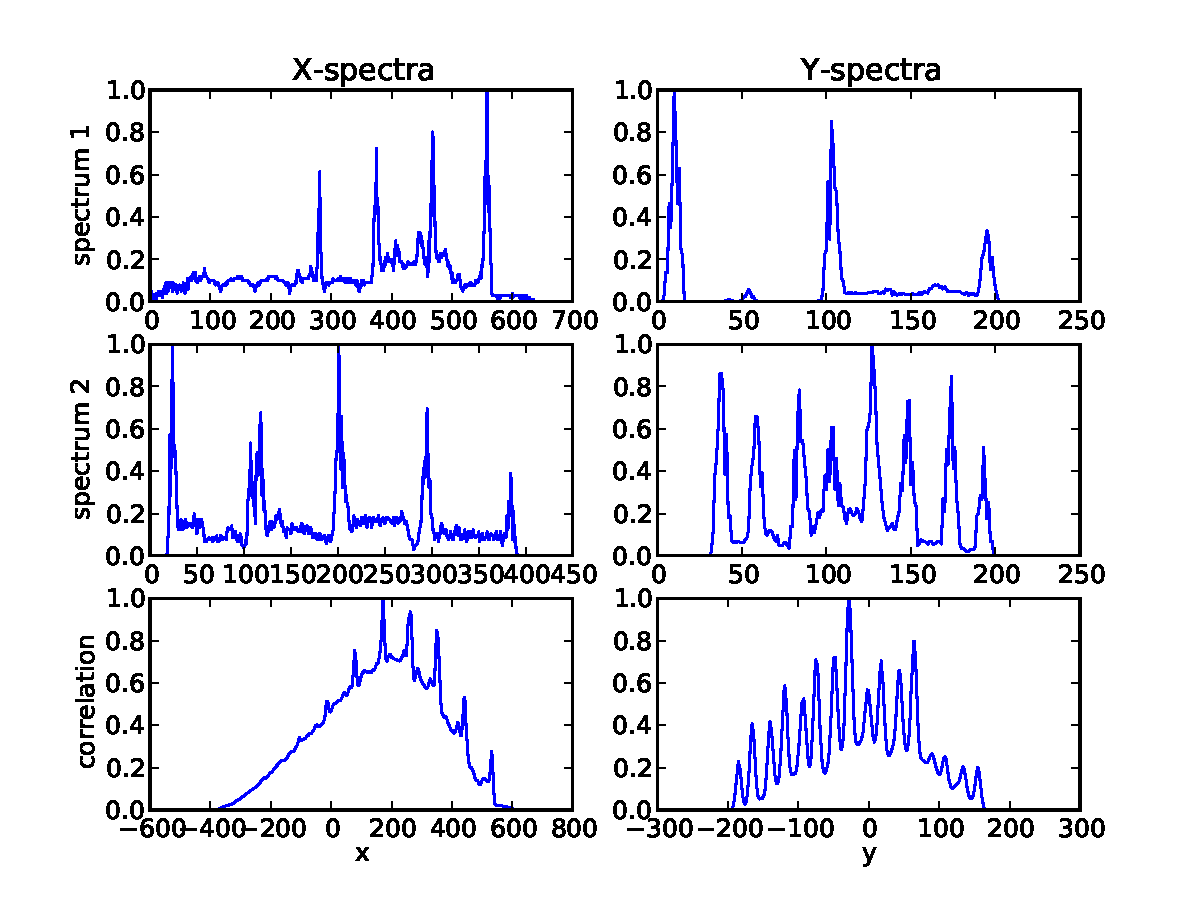
\includegraphics[width=0.8\textwidth]{images/experiment/map1/stitch1-1a-xy-correlation.pdf}
  \caption{Finding optimal translation $t$ through correlating Hough spectra.}
  \label{fig:exp:1:xy}
\end{figure}

\begin{figure}[ht]
  \centering
  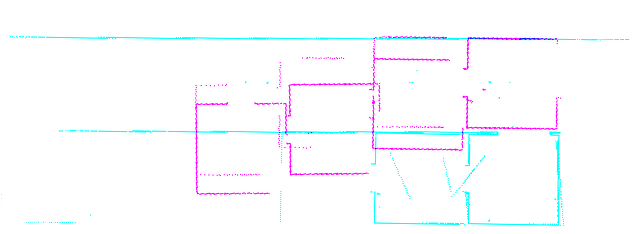
\includegraphics[width=0.8\textwidth]{images/experiment/map1/stitch1-1a-result.png}
  \caption{The best stitch according to $\theta_{1a}$ and optimal $t$.}
  \label{fig:exp:1:result1}
\end{figure}

The result of this stitch is far from optimal. While the rotation angle $\theta_{1a}$ is optimal and the images are rotated correctly, the translation estimate $t$ is very much off. The Hough-transform based map stitching method requires a large overlapping area between the two submaps. Because the submaps overlap very little, the stitching method fails.

In the next figure, \ref{fig:exp:1:result8}, the final result of stitching all submaps in figure~\ref{fig:apx:map1-pieces} is shown. Each of the steps is separately shown in the appendix (\ref{})

\begin{figure}[ht]
  \centering
  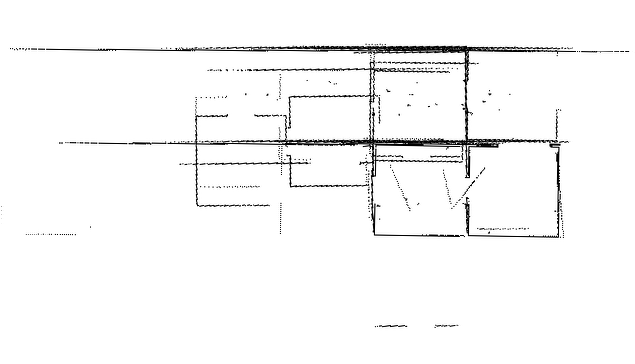
\includegraphics[width=0.8\textwidth]{images/experiment/map1/result/step8.png}
  \caption{The result of stitching all partial maps (see figure~\ref{fig:apx:map1-pieces}) according to the Hough stitching method. Compare to the original SLAM result, figure~\ref{fig:map1-map}.}
  \label{fig:exp:1:result8}
\end{figure}

\section{Map 2}
The second map is from the Dutch Open 2012, preliminary round 1. It features a large outdoor environment. This is extra challenging for the Hough transform based map stitching method, as this method requires straight lines which are not often present in outdoor environments.

** Something went wrong with the map pieces, they're from Map 3. I have to re-export them in the lab, monday :( **

%Places to break:
%[ 19  23  24  32  33  34  35  36  37  38 105 111 113 114 115 116 117 118
% 119 120 135 146 149 151 163 168 169 170 171 184 186 188 190 191 192 193
% 194 195 196 197 198 199 200 210 211 212 213 214 215 216]


% Decide to break only on one place, where a number of consecutive items do not match, and large enough patches result.

%show traces of the map

\section{Map 3}
The third map is again a map from the IranOpen 2012 championship. The map was used for the semi-final. It is rather large, and consists of many corridors and rooms filled with desks, chairs and computers. Some of the hallways are obstructed, and there is smoke everywhere. See figure~\ref{fig:map3-screenshot}.

\begin{figure}[ht]
\centering
  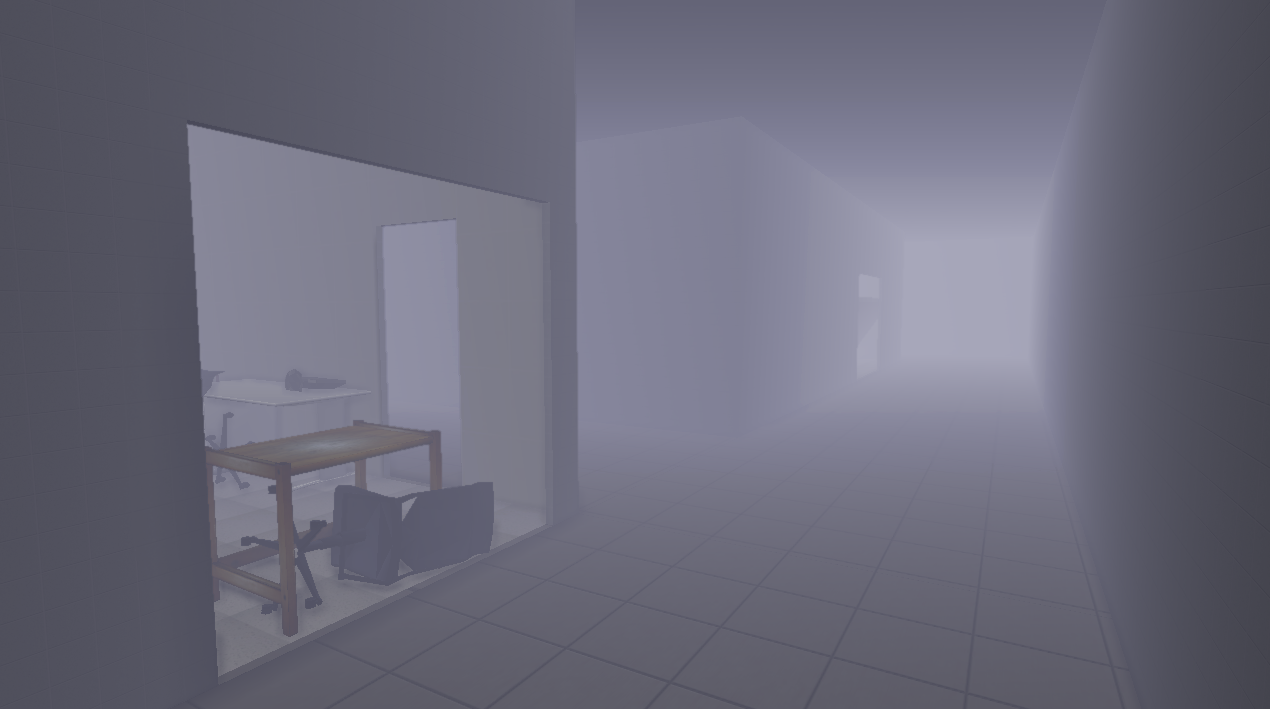
\includegraphics[width=0.5\textwidth]{images/experiment/map3/map3.png}
  \caption{A screenshot of map 3.}
  \label{fig:map3-screenshot}
\end{figure}

TODO: add the full SLAM result as well.

The agent was driven in a large circular path ($50m$ diameter) through the building, as can be seen in figure~\ref{fig:map3-trace}. Again, the path given by the inertia sensor seems to lie closer to the groundtruth than the SLAM path. The SLAM path strays on many places from the path by the inertia sensor and SLAM, and is `pulled back' to the location given by the inertia sensor when the difference becomes too large.

\begin{figure}[ht]
\centering
  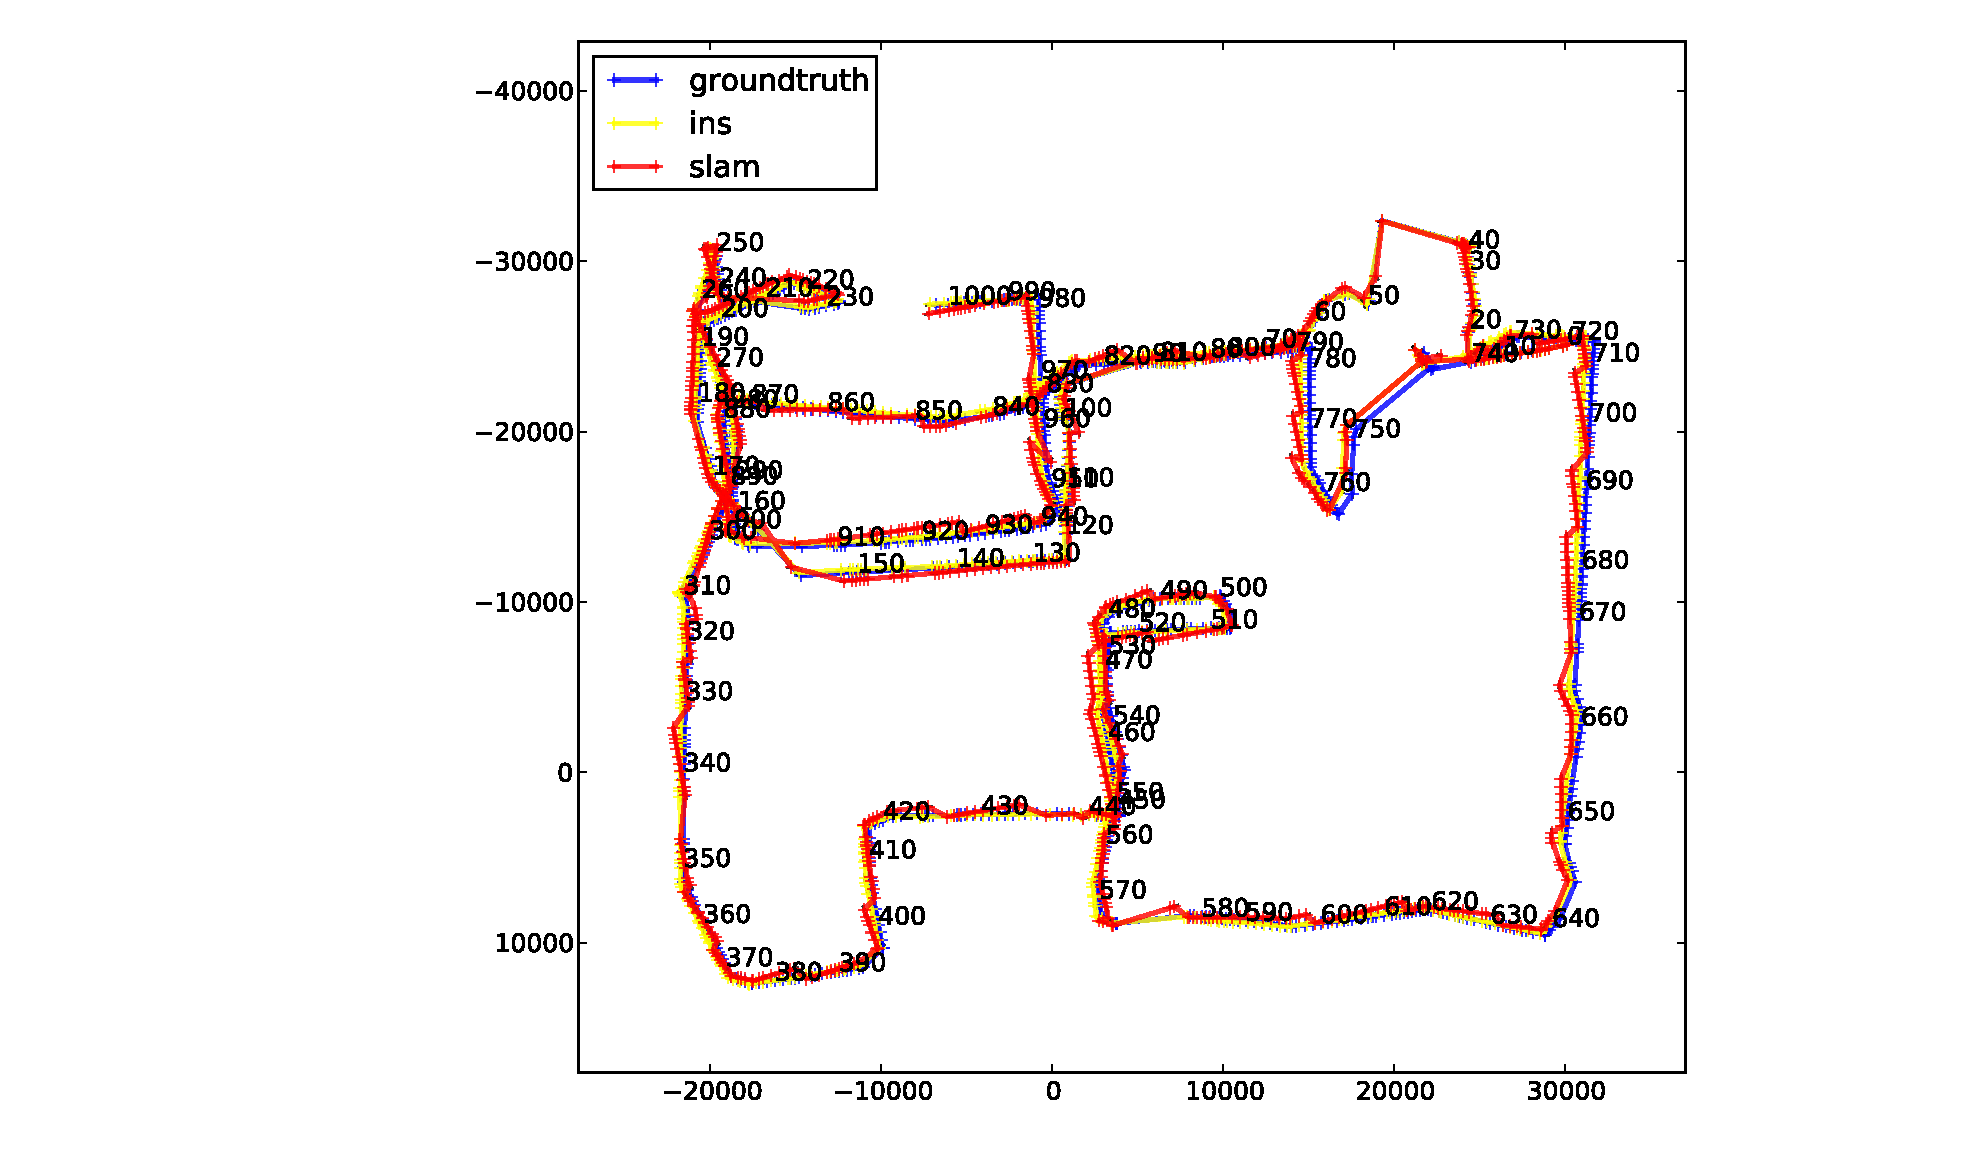
\includegraphics[width=\textwidth]{images/experiment/map3/trace2.pdf}
  \caption{The Ground Truth data, inertia sensor data and WSM slam result for map 3.}
  \label{fig:map3-trace}
\end{figure}

The error measures extracted from the Weighted Scan Matcher are shown in figure~\ref{fig:map3-confidence}. Just as in the previous experiments, there are a number of time steps where no matching scan lines were found. At these timesteps, the covariance matrix around the location estimate could not be computed, and are respresented by a red circle at the x-axis. Instead of segmenting the map at every timestep where the number of matches was zero, a different approach is tried for this experiment. The map is segmented on at those timesteps where there are 2 or more consecutive timesteps in which there were no matching scanlines. The resulting 3 submaps are shown in the appendix, figure~\ref{fig:apx:map3-pieces}.

\begin{figure}[ht]
\centering
  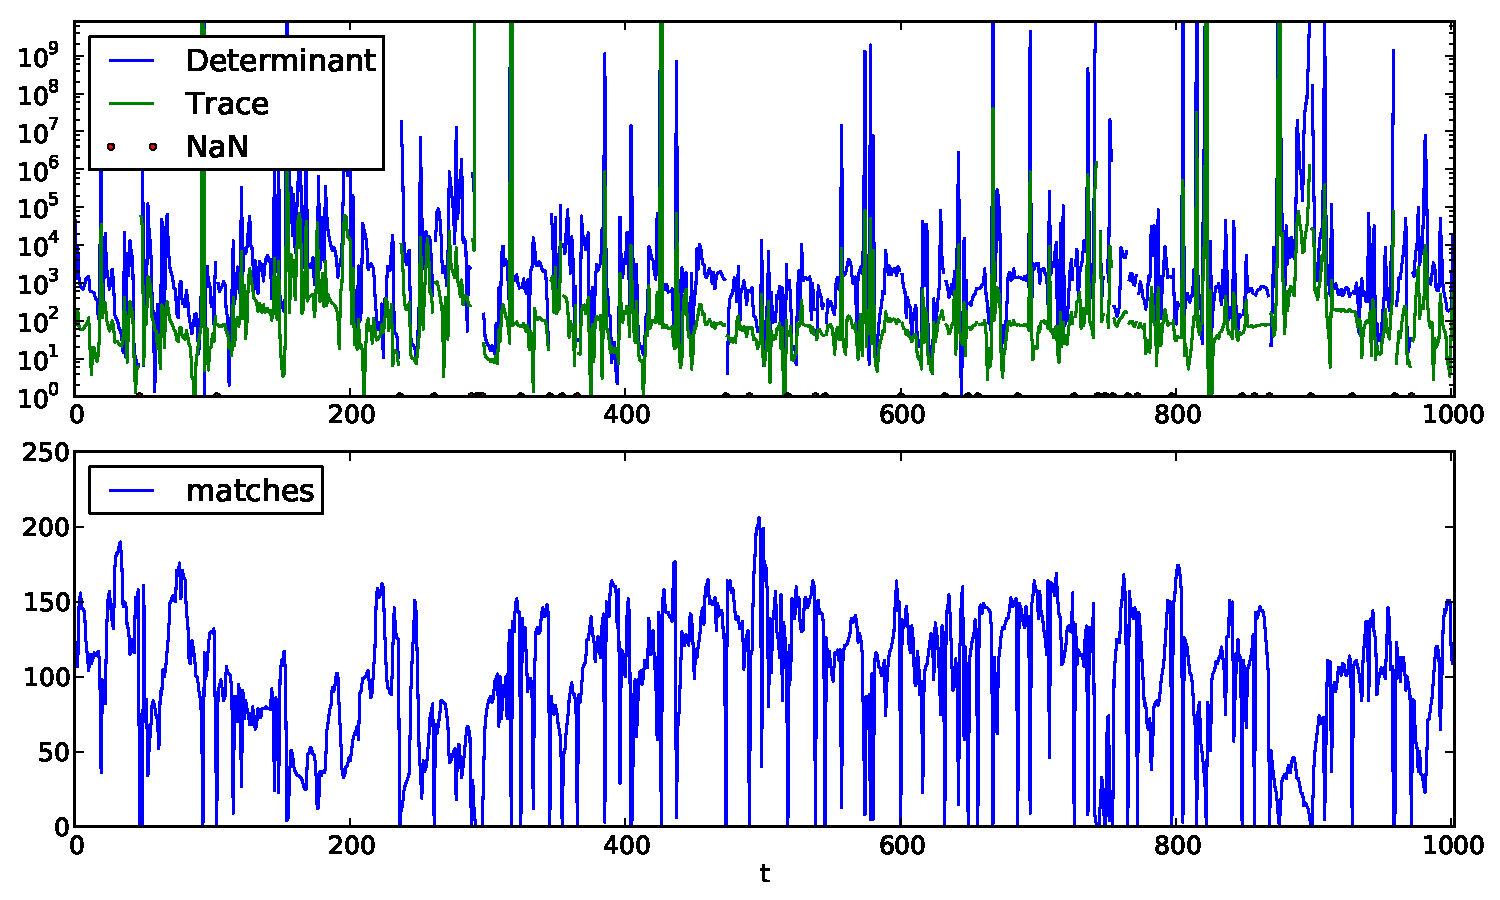
\includegraphics[width=\textwidth]{images/experiment/map3/error-measures.pdf}
  \caption{Confidence measures for map 3.}
  \label{fig:map3-confidence}
\end{figure}

The result of stitching the submaps with the Hough transform based stitching method can be inspected in figure~\ref{fig:map3-result}. As can be easily visually inspected, this result is much worse than the result by the manifold SLAM.

\begin{figure}[ht]
\centering
  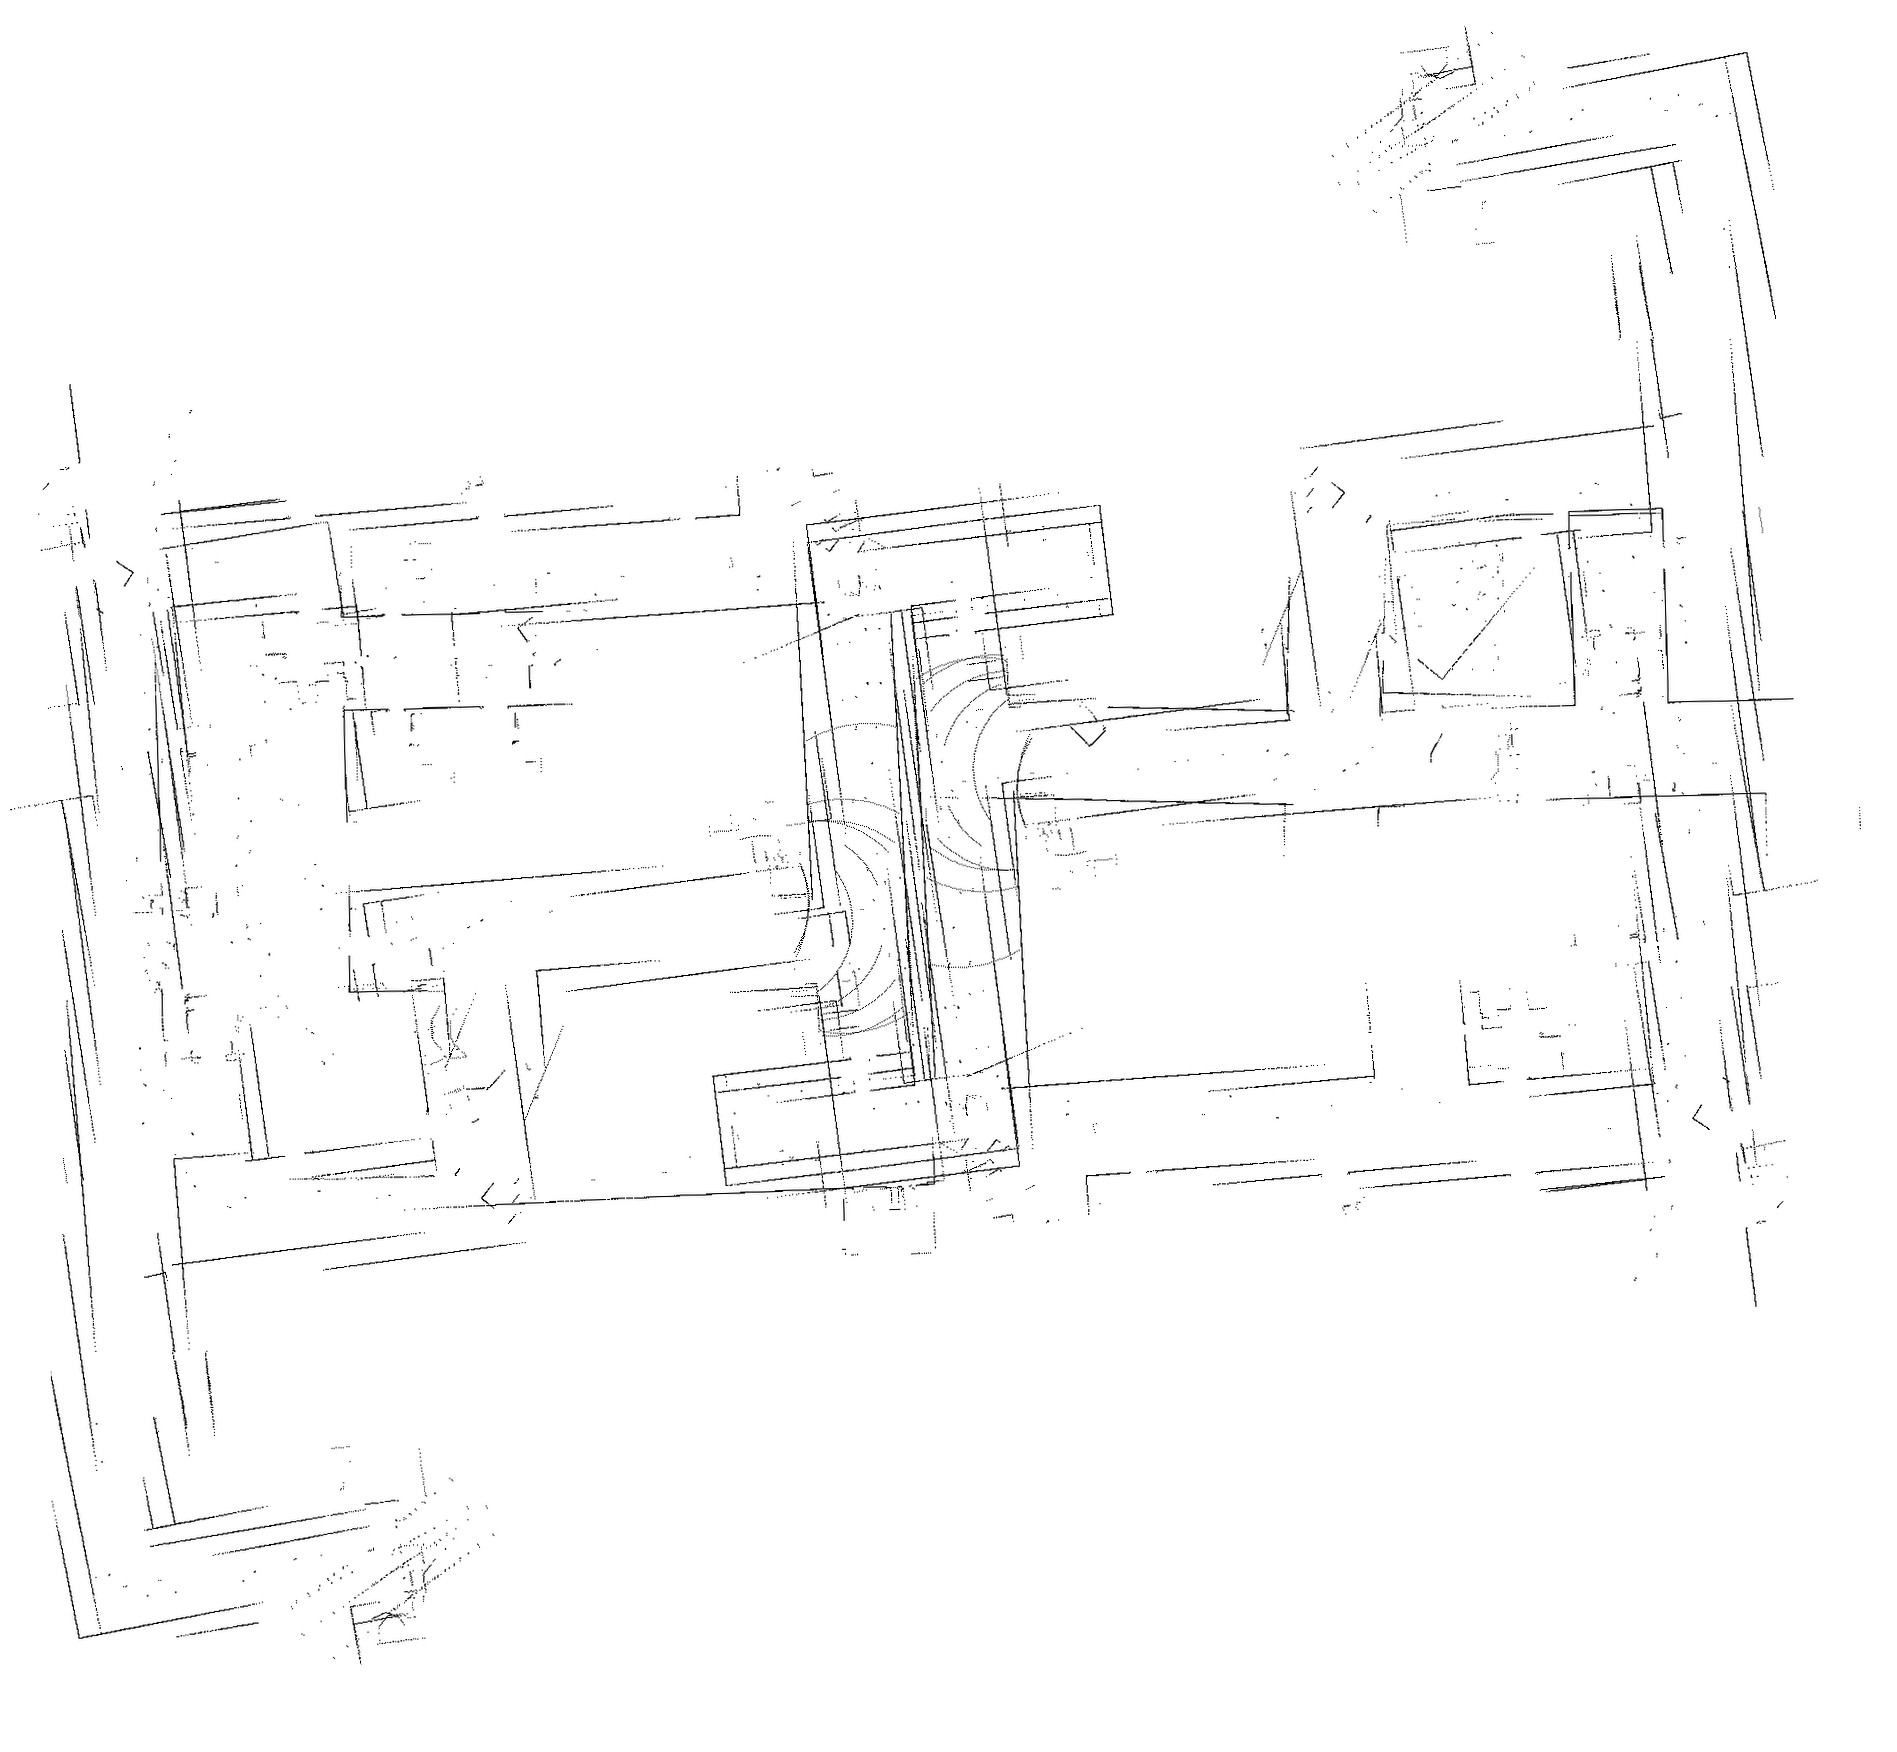
\includegraphics[width=\textwidth]{images/experiment/map3/result/step2.png}
  \caption{The resulting map after stitching all segments extracted from map 3.}
  \label{fig:map3-result}
\end{figure}


\section{Discussion of results}
** This is only a list of points that need to be discussed, need to be fleshed out **

The results show that the rotation can be guessed very nicely within a human-made environment by the Hough-transform. The translation estimate is not good.

The translation estimate might be done with a scanmatcher, when the rotation estimate is guessed by hough.

The overlap between patches needs to be large.

A smoother fitness landscape could improve alignment somewhat. This can be done by running a Gaussian filter.

The quality of the submaps should be very high before a good stitching can be done with the Hough transform. The results obtained through the Weighted Scan Matcher are 